\documentclass[letterpaper,twocolumn]{article}

\usepackage[top=0.5in, bottom=1in, left=1in, right=1in]{geometry}
\usepackage{float}
\usepackage{graphicx}
\usepackage{caption}
\usepackage{subcaption}
\usepackage{amsmath}
\usepackage{sectsty}
\sectionfont{\large}
\usepackage{todonotes}

\title{\large \textbf{Angular Motion Control Using a Closed-Loop CPG for a Water-Running Robot}}
\author{\small Nitish Thatte, Mahdi Khoramshahi, Metin Sitti \\
        \small Carnegie Mellon University \\
        \small \{nitisht, khoram\} at andrew.cmu.edu, metin at cmu.edu
}
\date{}
\begin{document}

\maketitle
\section{Motivation}
The Basilisk Lizard's striking ability to sustain highly dynamic legged locomotion on a range of surfaces from hard-ground to water is a remarkable feat \cite{glasheen1996hydrodynamic}. Most legged robots would have difficulty emulating this animal's ability to robustly locomote on yielding or deforming surfaces. Therefore, to explore the dynamics of legged locomotion in this regime, we are studying the design of a bio-inspired water-running robot. Analyzing water-running dynamics may also help us gain insight into mobility on other yielding surfaces, such as granular media and mud. It is crucial that we develop locomotion models for these surfaces as robots continue to venture out of the laboratory and into the real world.


\section{State of the Art}
The mechanical design of the water-running robot has undergone several design iterations. The current design, which can be seen in figure~\ref{fig:robot}, features four four-bar linkage legs producing  foot trajectories, as in figure \ref{fig:traj}, optimized for power consumption and lift. Park et al analyzed the roll and pitch dynamics of this robot and proposed an active tail for achieving stable robot pitch angles \cite{park2010roll}. However, addition of an active tail requires integration of another actuator, adding mass and complexity. Furthermore, no method for controlling roll angles has been proposed as of yet.




\section{Own Approach}
To control the roll and pitch motion of the robot, we propose a novel, closed-loop central pattern generator (CPG) that modulates the velocity of each foot during the downwards and upwards phases of their trajectories using a control input parameter we call duty-factor. This approach takes advantage of non-linear fluid drag to generate differing forces on each foot, thereby imparting moments on the robot. 
	
To deal with the hybrid and time-variant nature of the system we utilize a time averaging approach. We then find the force generated by an approximated foot trajectory in order to yield an expression, which is linear in duty-factor, for the average lift force over a cycle.  Finally, we design a controller, based on this force equation, to achieve a desired spring-like virtual model.


\begin{figure}[tb]
	\centering
	\begin{subfigure}[c]{0.24\textwidth}
		\centering
		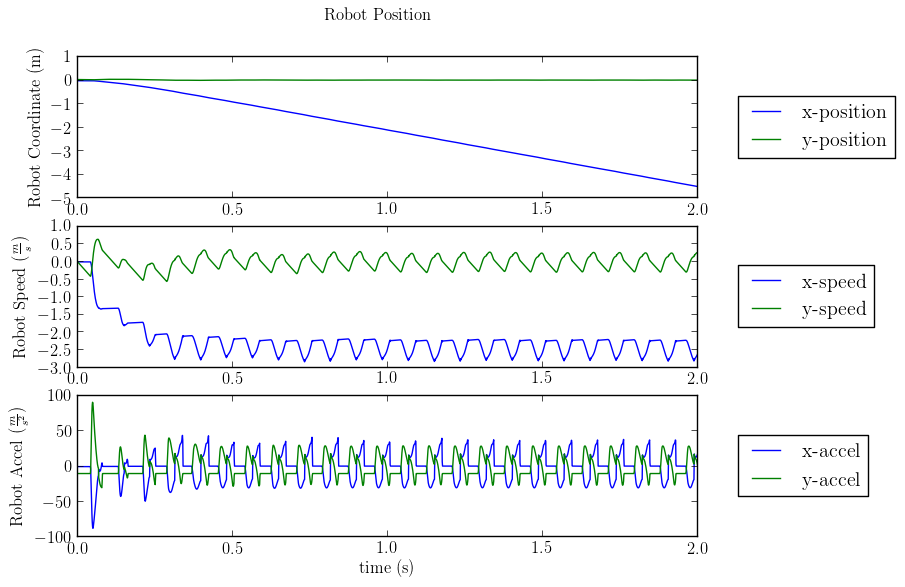
\includegraphics[width = \textwidth]{figures/robot.png}
	\end{subfigure}
	\begin{subfigure}[c]{0.24\textwidth}
		\centering
		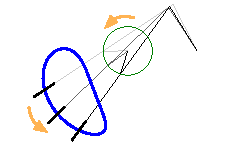
\includegraphics[width = \textwidth]{figures/traj.pdf}
	\end{subfigure}

	\begin{subfigure}[c]{0.24\textwidth}
		\caption{Robot Design}
		\label{fig:robot}
	\end{subfigure}
	\begin{subfigure}[c]{0.24\textwidth}
		\caption{Foot Trajectory}
		\label{fig:traj}
	\end{subfigure}
	\vspace{-0.25in}
	\caption{}
	\vspace{-0.15in}
\end{figure}

\section{Current Results}
In order to control the roll and pitch angles of the robot, we must be able to control the height of each corner of the robot. We have achieved preliminary results controlling the height of a one legged hopping robot using the nonlinear control outlined in the previous section. We have found that adding PID to this control scheme in an outer loop can reduce setting time, oscillations about the desired height, and steady state error.


\section{Best Possible Outcome}
We will extend the height controller described above to control roll and pitch angles. We will then use this controller to control the roll and pitch angles of the water-runner robot in simulation. These simulated experiments will then be validated on the real robot.


\section*{Acknowledgment}
This material is based upon work supported by the National Science Foundation Graduate Research Fellowships. 

\bibliographystyle{plain}
\bibliography{dynamic}

\end{document}
